% (c) Egor Osipov

\documentclass[a4paper,12pt]{article} % тип документа (report, book)
\usepackage[14pt]{extsizes}
\usepackage[left=2cm,right=2cm, top=2cm,bottom=2cm,bindingoffset=0cm]{geometry} % Настройки документа
\usepackage{pgfplots}
\usepackage{pgfplotstable}
\usepackage{tikz} 

%  Русский язык
\usepackage[T2A]{fontenc}			% кодировка
\usepackage[utf8]{inputenc}			% кодировка исходного текста
\usepackage[english,russian]{babel}	% локализация и переносы


% Математика
\usepackage{amsmath,amsfonts,amssymb,amsthm,mathtools} 

% Просто смайлики
\usepackage{wasysym}

%Вставка картинок
\usepackage{graphicx}
\graphicspath{./}
\DeclareGraphicsExtensions{.pdf,.png,.jpg}
\usepackage{float}

% Настройка абзацев
\usepackage{indentfirst}
%\setlength{\parindent}{5ex}
%\setlength{\parskip}{1em}

\begin{document} % начало документа

%Заговолок
\begin{titlepage}
\begin{center}
	\large{Московский физико-технический институт}\\
	\vspace{100px}
	\LARGE{Работа 4.4.3}\\
	\LARGE{Изучение призмы с помощью гониометра.}\\
	\vspace{30px}
	
\includegraphics[scale = 0.3]{fakt_logo.png}\\
\end{center}

\vfill
\begin{flushright}
	\text{Осипов Егор. Б03-005}\\
	\text{г. Долгопрудный}
\end{flushright}
\end{titlepage}

\newpage

\tableofcontents

\newpage

\section{Цель работы и приборы.}

\textbf{Цель работы:} знакомство с работой гониометра, исследование дисперсии стеклянной призмы и определение характеристик призмы как спектрального прибора.

\textbf{В работе используются:} гониометр, ртутная лампа, призма, стеклянная плоскопараллельная пластинка, призменный уголковый отражатель.

\section{Теоритическая вводная.}

Гониометр служит для точного измерения углов и находит широкое применение в оптических лабораториях. С помощью гониометра можно определять показатели преломления и преломляющие углы призм и кристаллов, исследовать параметры дифракционных решёток, измерять длины волн спектральных линий и т. д. В настоящей работе прибор применяется для исследования дисперсии стеклянных призм --- зависимости показателя преломления от длины волны.

\begin{figure}[H]
\noindent\centering{
\hspace{-0mm}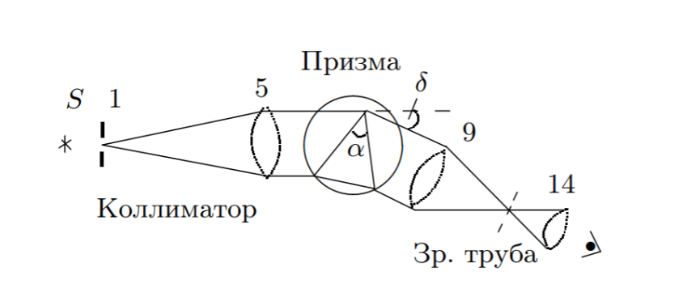
\includegraphics[scale = 0.5]{pic1}
}
\caption{Оптическая схема эксперимента.}
\label{pic1:ref}
\end{figure}

Показатель преломления материала призмы удобно определять по углу наименьшего отклонения. Известно, что минимальное отклонение луча, преломленного призмой, от направления луча, падающего на призму, получается при симметричном ходе луча (в призме луч идёт перпендикулярно биссектрисе преломляющего угла). Угол минимального отклонения $\delta$, преломляющий угол $\alpha$ (угол при вершине призмы на рис. 1) и показатель преломления $n$ связаны между собой соотношением

\begin{equation}
	n=\dfrac{\sin\dfrac{\alpha+\delta}{2}}{\sin\dfrac{\alpha}{2}}.
\end{equation}

Измерив с помощью гониометра преломляющий угол призмы и углы наименьшего отклонения для света разных длин волн, можно рассчитать величину $n$ и построить дисперсионную кривую --- график зависимости $n(\lambda)$. 

	По дисперсионной кривой могут быть определены такие важные характеристики оптических стёкол, как средняя дисперсия

\begin{equation}
	D = n_F - n_C
	\end{equation}

и коэффициент дисперсии $\nu$ (число Аббе):
	\begin{equation}
	\nu = \dfrac{n_D - 1}{n_F - n_C},
	\end{equation}
	где $n_D, n_F$ и $n_C$ --- показатели преломления для $\lambda_D = 589{,}3$ нм (среднее значение длин волн жёлтого дублета натрия), $\lambda_F = 486{,}1$ нм (голубая линия водорода), $\lambda_C = 656{,}3$ нм (красная линия водорода).
	
	По наклону дисперсионной кривой можно оценить разрешающую
	способность призмы
	\begin{equation}
	R = \dfrac{\lambda}{\delta\lambda} = b\dfrac{dn}{d\lambda}.
	\end{equation}
	Здесь $\delta\lambda$ --- минимальный интервал длин волн, разрешаемый по критерию Релея, $b$ --- размер основания призмы, если вся рабочая грань призмы освещена параллельным пучком.
	
		\begin{figure}[h]
		\begin{center}
			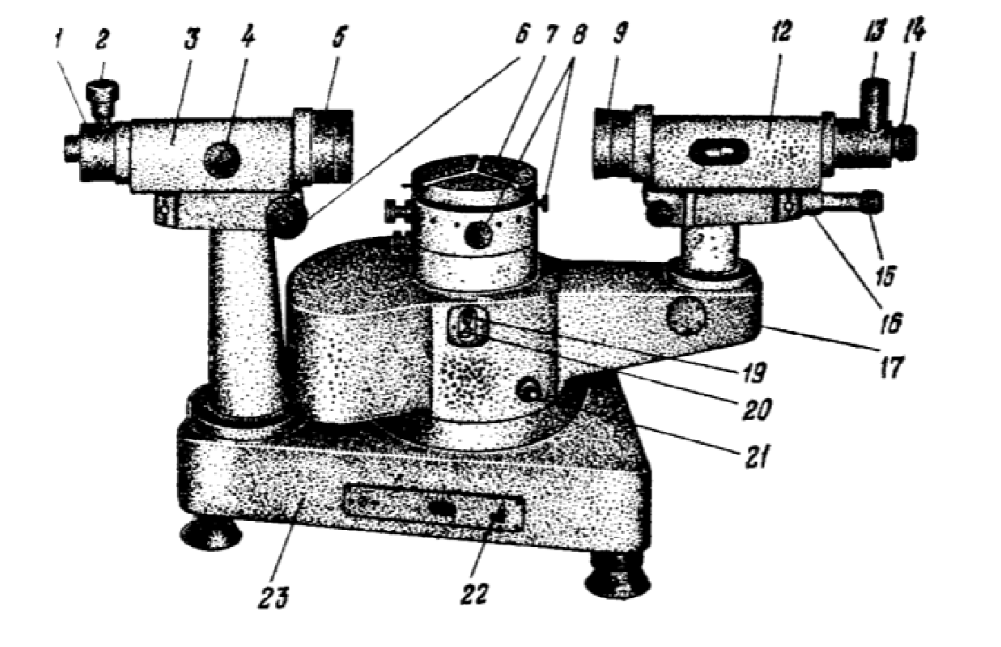
\includegraphics[width = 0.9\textwidth]{pic2}
			\caption{Внешний вид гониометра}
		\end{center}
	\end{figure}
	
	\section{Ход работы}
	В работе предлагается отъюстировать гониометр, определить преломляющий угол призмы, измерить углы наименьшего отклонения для нескольких спектральных линий ртути и оценить спектральные характеристики призмы.
	\subsection{Юстировка гониометра и установка призмы}
	\begin{enumerate}
		\item Поворачивая столик рукой, установили его на глаз горизонтально при помощи двух винтов, ориентированных взаимно перпендикулярно. Установили зрительную трубу на бесконечность и поверхность столика перпендикулярно оси вращения прибора. Настроили колиматор, подобрали рабочую ширину входной щели так, чтобы её видимая ширина составляла 1,5–2 расстояния между полосами двойного отсчётного штриха. Установили начало отсчёта в $0^\circ1'00''$.
		
		\item Поставили рабочую призму так, чтобы её преломляющее ребро было вертикально, а одна из рабочих граней была перпендикулярна одному из установочных винтов, подстроили столик и отрегулировали винты.
	\end{enumerate}
	
	\subsection{Измерение преломляющего угла}
	\begin{enumerate}
		\item Для определения минимального угла отклонения $\delta$ поставили призму на столике так, чтобы её основание было параллельно оси коллиматора (на глаз). Расположили лист бумаги за призмой и нашли на нём спектр, вращая столик рукой. Продолжая поворачивать столик и наблюдая за перемещением спектра, нашли положение столик а с призмой, соответствующее минимальному отклонению преломлённого луча от направления падающего луча.
		
		\item Нашли спектр и зрительную трубу, настроились на одну из жёлтых линий (см. рис. 3 и табл. 1) и, вращая столик сначала рукой, а затем винтом тонкой подачи, установили его в такое положение, при котором отклонение выбранной спектральной линии от направления оси коллиматора оказывается наименьшим.		
		\begin{figure}[h]
			\begin{center}
				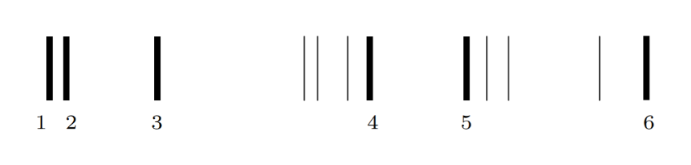
\includegraphics[width = 0.55\textwidth]{pic3}
				\caption{Спектр ртутной лампы ДРШ--250}
			\end{center}
		\end{figure}
	\begin{table}[]
		\centering
		\begin{tabular}{|c|c|c|c|c|c|c|c|c|}
			\hline
			№ & $K_1$ & $K_2$ & 1 & 2 & 3 & 4 & 5 & 6 \\ \hline
			$\lambda,$ нм & 690,7 & 623,4 & 579,1 & 577,0 & 546,1 & 491,6 & 435,8 & 404,7 \\ \hline
			Цвет &красн.&красн.& желт. & желт. & зелен. & голуб. & синий & фиолет. \\ \hline
			Яркость & 4 & 4&10 & 8 & 10 & 4 & 4 & 3 \\ \hline
		\end{tabular}
		\caption{Характеристики спектра ртутной лампы ДРШ--250}
		\label{tab:my-table}
	\end{table}
	\item Вращая алидаду сначала от руки при освобождённом винте, а затем винтом тонкой подачи при закреплённом винте, совместили двойной штрих измерительный сетки с выбранной линией и сняли отсчёт по лимбу. Для каждой линии спектра (рис. 3) нашли минимум отклонения (своё положение столика с призмой) и определили координату линии:
	\begin{center}
		\centering
		\begin{tabular}{|c|c|c|c|c|c|}
			\hline
			№ & $K_1$ & $K_2$ & 1 & 2 & 3  \\ \hline
			$\delta$ & $51^\circ00'49''$ & $51^\circ37'25''$ & $52^\circ01'15''$ & $52^\circ02'14''$ & $52^\circ22'32''$ \\ \hline
		\end{tabular}
	
	\begin{tabular}{|c|c|c|c|}
		\hline
		№ & 4 & 5 & 6 \\ \hline
		$\delta$  & $53^\circ09'17''$ & $54^\circ20'46''$ & $55^\circ19'26''$ \\ \hline
	\end{tabular}
	\end{center}
	\end{enumerate}
	\subsection{Разрешающая способность}
	Для оценки разрешающей способности призмы измерили угловую ширину жёлтых линий дублета, предварительно установив минимально возможную ширину входной щели:
	\begin{center}
		\begin{tikzpicture}
		\fill[fill=black!20] (0,0) -- (-1.5,0) -- (-1.5,2) -- (0,2);
		\fill[fill=black!20] (1.2,0) -- (0.7,0) -- (0.7,2) -- (1.2,2);
		\fill[fill=black!20] (1.8,0) -- (3.3,0) -- (3.3,2) -- (1.8,2);
		\draw[dashed] (0,0) -- (0,2);
		\draw[dashed] (0.7,0) -- (0.7,2);
		\draw[dashed] (1.2,0) -- (1.2,2);
		\draw[dashed] (1.8,0) -- (1.8,2);
		\fill (0,1) circle (0.05) node[left] {$x_0$};
		\fill (0.7,1) circle (0.05) node[above left] {$x_1$};
		\fill (1.2,1) circle (0.05) node[above right] {$x_2$};
		\fill (1.8,1) circle (0.05) node[right] {$x_3$};
		\end{tikzpicture}
		\\
		\vspace{0.4cm}
		\begin{tabular}{|c|c|c|c|}
			\hline
			$x_0$ & $x_1$ & $x_2$ & $x_3$ \\ \hline
			$7'15''$  & $6'41''$ & $5'54''$ & $5'24''$ \\ \hline
		\end{tabular}
	\end{center}
	Измерили линейкой длину $b=7{,}4\pm0{,}1$ см основания призмы.

\section*{Обработка результатов}
\begin{enumerate}
	\item Рассчитали минимальные углы отклонения $\delta(\lambda)$ и показатель преломления $n(\alpha,\delta)$ по формуле (1) и построили дисперсионную кривую $n(\lambda)$:

	\begin{center}
	\begin{tabular}{|c|c|c|c|c|c|c|c|c|}
		\hline	
		$\lambda,$ нм & 690,7 & 623,4 & 579,1 & 577,0 & 546,1 & 491,6 & 435,8 & 404,7 \\ \hline
		$n,$ нм & 1,6484&1,6544&1,6583&1,6584&1,6617&1,6693&1,6806&1,6898 \\ \hline
	\end{tabular}
	\end{center}	
	
\begin{figure}[h]
		\begin{center}
			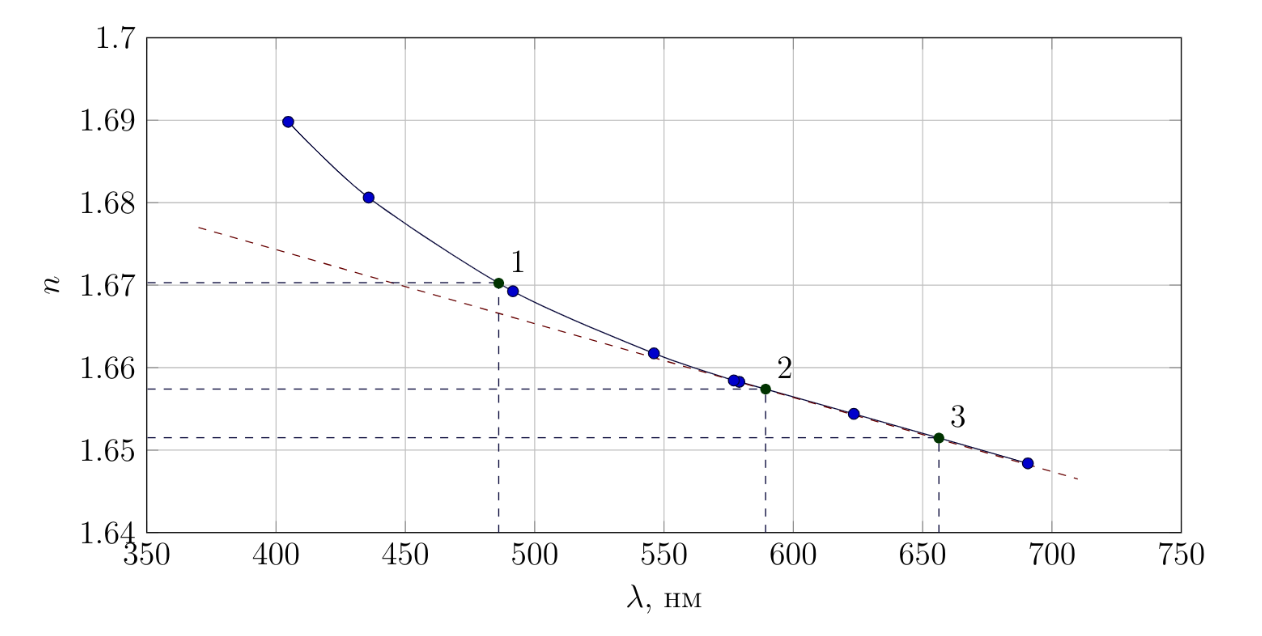
\includegraphics[width = 0.9\textwidth]{graph}
			\caption{Дисперсионная кривая.}
		\end{center}
	\end{figure}

	
	\textit{Комментарий по поводу погрешностей в эксперименте:} погрешность угла призмы неизвестна, но стоит полагать, что она на несколько порядков больше погрешности измерений, то есть $0^\circ0'1''$. При этом для построения графиков и дальнейших рассчётов по ним, вероятно, обе погрешности не имеют значения, так как не разрешаются на бумаге.
	
	\item Определили по графику 
	\begin{equation*}
	n_D = 1{,}658\pm0{,}001,\;\;\;n_F = 1{,}670\pm0{,}001,\;\;\;n_C = 1{,}652\pm0{,}001,
	\end{equation*}
	и рассчитали среднюю дисперсию стекла по формуле (2):
	\begin{equation*}
		D = n_F - n_C = 0{,}018\pm0{,}002.
	\end{equation*}
	При определении $n_C$ с помощью спектра ртутной лампы дисперсионную кривую приходится несколько экстраполировать в область длинных волн. Рассчитали число Аббе по формуле (3)
	\begin{equation*}
	\nu = \dfrac{n_D - 1}{n_F - n_C} = 36\pm 4,
	\end{equation*}
	 и определили по таблицам сорт стекла --- предположительно баритовый флинт.
	 	\begin{figure}[h]
	 	\begin{center}
	 		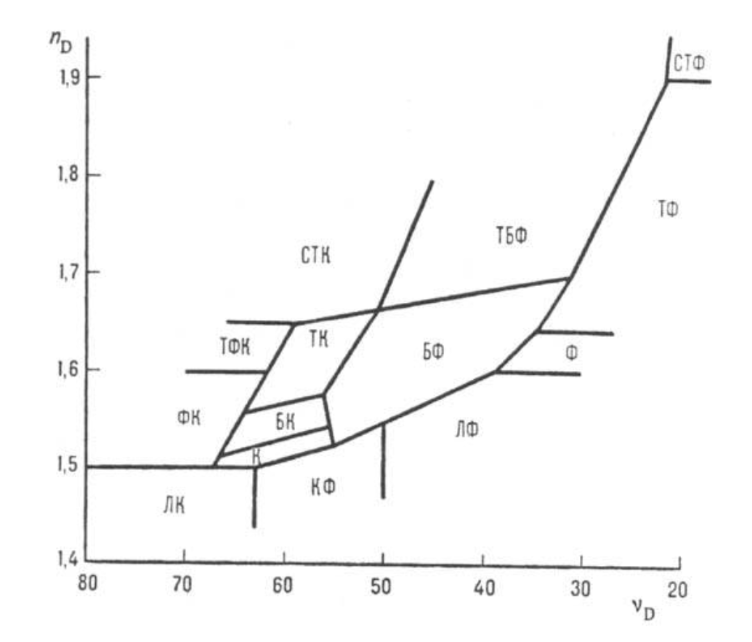
\includegraphics[width = 0.6\textwidth]{pic4}
	 		\caption{\small{Диаграмма Аббе: ЛК — лёгкие кроны; ФК — фосфатные кроны; ТФК — тяжёлые фосфатные кроны; К — кроны; БК — баритовые кроны; ТК — тяжёлые кроны; КФ — кронфлинты: БФ — баритовые флинты; ТБФ — тяжёлые баритовые флинты; ЛФ — лёгкие флинты; Ф — флинты; ТФ — тяжёлые флинты; СТФ — сверхтяжёлые флинты; СТК — сверхтяжёлые кроны.}}
	 	\end{center}
	 \end{figure}
	\item По наклону кривой $dn/d\lambda = (8{,}9\pm0{,}5)\cdot10^{4}\text{ м}^{-1
	}$  рассчитали максимальную разрешающую способность призмы по формуле (4):
	\begin{equation*}
	R = b\dfrac{dn}{d\lambda} = 6700\pm500.
	\end{equation*}
	Рассчитали экспериментальную величину $R$ по измерениям жёлтого дублета:
	\begin{equation*}
	R > \dfrac{\lambda}{\delta\lambda} \approx 275.
	\end{equation*}
	
	Оценили, при каком размере решётки, имеющей 100 штр/мм, она обладает такой же разрешающей способностью в первом порядке, как призма с основанием $b = 5$ см.
	\begin{equation*}
	a\cdot100\text{ штр./мм} = R = b\dfrac{dn}{d\lambda},
	\end{equation*}
	\begin{equation*}
	a = 44\pm3 \text{ мм}.
	\end{equation*}
	\item Рассчитали угловую дисперсию $d\phi/d\lambda = 0{,}0126\pm0{,}0006\text{ }^\circ\text{/нм}$ и по измерениям жёлтого дублета и сравнили её с дисперсией решётки в первом порядке, имеющей 100 штр/мм:
	\begin{equation*}
	D = \dfrac{1}{100\text{ штр./мм}} = 0{,}01\text{ мм} = 5{,}73\cdot10^5\text{ }^\circ\text{/нм}.
	\end{equation*}
\end{enumerate}

\section{Вывод}
Ознакомились с работой гониометра, исследовали дисперсию света ртутной лампу на стеклянной призме. По измеренным данным определили показатели преломления для длин волн жёлтого дублета натрия, голубой и красной линий водорода. Также оценили разрешающую способность призмы, рассчитали среднюю дисперсию стекла. По полученным значениям сделали предположение о сорте стекла. Сравнили разрешающую способность и угловую дисперсию призмы с соответствующими параметрами дифракционной решётки.
\end{document}

\end{document} % конец документа
